% vim: set tw=78 sts=2 sw=2 ts=8 aw et ai:

Topic models specify a mixture of topics for each historically relevant document and thus for each year. The analysis of all variants of relevance has shown that only rarely does a year fail to have a dominant topic (over $50 \%$), so only the most likely topic for each year shall be considered.

\begin{figure*}[ht]
\centering
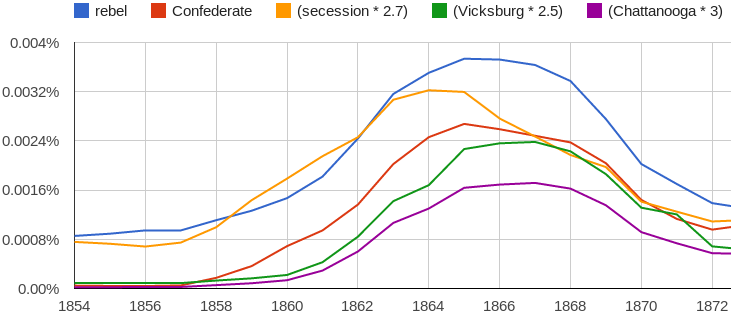
\includegraphics[max size={0.7 \textwidth}{0.7 \textheight}]{civil-war-related-series}
\caption{Ngram time series related to the American Civil War}
\label{fig:civil-war-related-series}
\end{figure*}

Though seemingly the weakest model, the double change algorithm has generated some of the most accurate topics for certain periods of time. For example, the topic for the years $1858$ to $1864$ and $1867$ to $1868$ is composed of the following main words: rebel, confederate, wolff, mcclellan, schleswig, secession, ich, vicksburg, rebels, chattanooga, die, sherman, doge, nicht, wedgwood, holstein, longstreet, gen, flax and der. A lot of these words relate directly to the American Civil War (see Figure~\ref{fig:civil-war-related-series}), providing a high degree of confidence that the model has successfully detected this important event in history.

\begin{figure*}[ht]
\centering
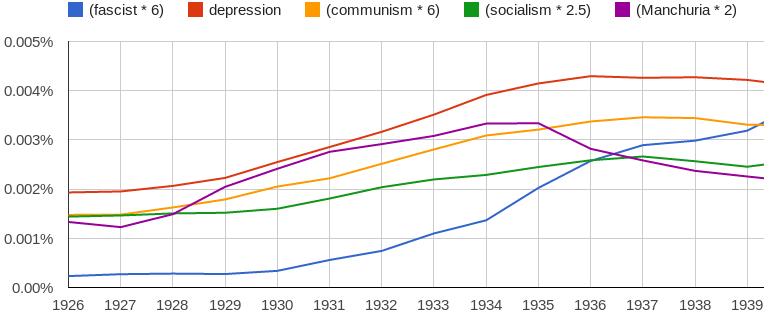
\includegraphics[max size={0.7 \textwidth}{0.7 \textheight}]{pre-ww2-related-series}
\caption{Ngram time series related to the pre World War II period}
\label{fig:pre-ww2-related-series}
\end{figure*}

For the linear model peak detection, the time period under consideration spans from $1932$ to $1936$, filled with events that foreshadowed World War II. The detected topic consists of fascist, adjustment, federal, depression, rubber, communism, collective, pact, medieval, vitamin, broadcasting, reconstruction, alpha, recovery, radio, employers, socialism, communists, tomorrow and manchuria. Unlike the case of the American Civil War, there is no underlying important event that could cause the topic to converge. Nonetheless, the selected words, the most relevant of which are shown in Figure~\ref{fig:pre-ww2-related-series}, do a good job of painting an accurate image of that period.

\begin{figure*}[ht]
\centering
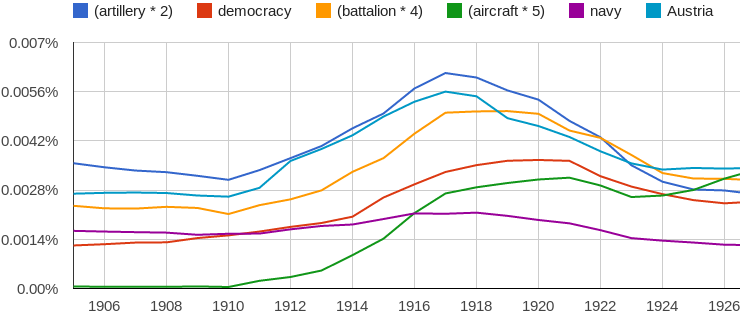
\includegraphics[max size={0.7 \textwidth}{0.7 \textheight}]{ww1-related-series}
\caption{Ngram time series related to World War I}
\label{fig:ww1-related-series}
\end{figure*}

For the last model, Gaussian model peak detection, the interval between $1916$ and $1920$ has a topic consisting of: artillery, target, syndrome, nationalism, naval, democracy, alcohol, battalion, pan, rehabilitation, defense, dad, von, aircraft, navy, strategic, austria, damping, mobilize and firing. The words pertaining to World War I are shown together in Figure~\ref{fig:ww1-related-series}.

\begin{table}[h]
\begin{center}
\begin{tabular}{|l|c|}
\hline \bf Year interval & \bf Topic words \\ \hline
\multirow{2}{*}{1899-1905} & electron, colonialism, \\
	& industrialization \\ \hline
1906-1912 & socialism, communism, korean \\ \hline
\multirow{3}{*}{1913-1921} & nationalism, artillery, \\
	& democracy, rehabilitation, naval \\
	& aircraft, hungary \\ \hline
\multirow{2}{*}{1922-1928} & petroleum, overseas, \\
	& gravitation, lagos \\ \hline
\multirow{2}{*}{1929-1935} & television, cinema, \\
	& capitalism, airport \\ \hline
\multirow{2}{*}{1936-1941} & semiconductor, ethiopian, \\
	& thermodynamic \\ \hline
\multirow{2}{*}{1942-1948} & aircraft, liberation, \\
	& victory, electronics \\ \hline
1949-1955 & spatial, seoul, charter \\ \hline
1956-1968 & rocket, disarmament, tibet \\ \hline
\multirow{2}{*}{1969-1981} & pollution, nixon, slavery, \\
	& blacks, urbanization \\ \hline
\multirow{2}{*}{1982-2007} & privatization, nicaragua, \\
	& ibm, nato, nuclear \\
\hline
\end{tabular}
\end{center}
\caption{\label{tbl:topic-evolution} Evolution of topics over the last century. }
\end{table}

However, many of the words present in these topics convey little information about a historic event, creating a significant amount of noise. Currently, their removal is done manually, but automating this task will most likely become the target of future research. An example of historic topics, describing the last century, can be seen in Table~\ref{tbl:topic-evolution} (obtained using the Gaussian model with a widening parameter $w = 2$).
